\documentclass[a4paper,11pt,twocolumn]{article}
\usepackage{mathtools}
\usepackage{esvect}
\usepackage{hyperref}
\usepackage{titling}

\setlength{\droptitle}{-10em}

\setlength{\intextsep}{6pt plus 1.0pt minus 2.0pt}

\title{Self-Organizing Map Implementation and Application (Lab 2)}

\date{November 28, 2017}

\author{
  Samuil Dichev, mbaxtsd2\\
  \texttt{The University of Manchester}\\
  \TextField{Lab Machine}\\
}

\begin{document}

\maketitle

\section{SOM Implementation}
Implementation begins by randomizing the position of $N$ neurons. For 1D SOM, they are arranged in a chain and the total amount is passed to the program. For 2D SOM, the total amount is equal to the $height * width$ of the lattice of neurons, which are given separately.

For each iteration (or training step), the algorithm randomly selects a data point. In our case, the data is arranged in a ring as shown in Figures \ref{fig:1d} and \ref{fig:2d}. For the selected data point, the algorithm determines the closest neuron (The winner or the Best Matching Unit (BMU)) using the Euclidean norm \[d_e(w,x) = ||w - x|| = \sqrt{(w - x)^T(w-x)}\] where in our case $w$ is the neuron vector and $x$ is the data point vector.

Next, the distance from the BMU to every other neuron is calculated to determine which neurons are within the neighbourhood, i.e. the radius of the BMU. This time, Manhattan distance is used, which is simply the sum of the absolute values of the differences between the coordinates for the 2D SOM or just the difference between indexes in the chain for the 1D SOM. Manhattan distance calculates the distance between two neurons in the lattice or in other words, how many hops along the lines in the lattice are needed to get from one neuron to another.
If a neuron is within the neighbourhood, the weight, i.e. coordinates of the neuron are updated as follows: \[w_i = w_i + L(t)\Theta(t)(x - w_i) \] where $x$ is the vector of the data point, $w_i$ is the vector of weight of the current neuron, $L(t)$ is the learning rate at the current iteration, $\Theta(t)$ is the result of the neighbourhood kernel function used to estimate how large of an adjustment to the weight should be made based on how far away from the BMU the current neuron is. This allows us to make smaller adjustments for neurons which are further from the BMU and larger adjustments for the neurons closer to the BMU. This is calculated as follows: \[\Theta = exp(-\frac{d^2}{2\sigma^2(t)}) \] where $d$ is the distance between the BMU and the current neuron and $\sigma(t)$ is the neighbourhood size at the current iteration. 

Finally, both the learning rate and neighbourhood size (or radius) are decreased by an exponential decay function respectively:
\[L(t) = L_0exp(-\frac{t}{\tau_1}) \]
\[\sigma(t) = \sigma_0exp(-\frac{t}{\tau_2}) \]

where $t$ is the current iteration (or time step) and $\tau_1$ and $\tau_2$ are parameters, which may be worth configuring for best results. In my implementation $\tau_1 = \tau_2 = trainingSteps$

Finally, we can see the results in Figures \ref{fig:1d} and \ref{fig:2d}. In both cases, the neurons closely follow the shape of the ring. We can see a gap between the first and last neuron in both the chain and the lattice. This is likely due to the fact that we are using Manhattan distance to calculate closeness. If a data point is selected at random during the algorithm training, which happens to be located right in that gap and one of the neurons at either end of the lattice becomes the BMU (winner), upon the update of its neighbours, the neuron at the other end will not update despite it being physically close, because it's far in the lattice. This would be different if we used Euclidean distance to determine neighbours, but Manhattan distance only considers distance in the lattice, not physical distance.

\begin{figure}[!h]
  \centering
  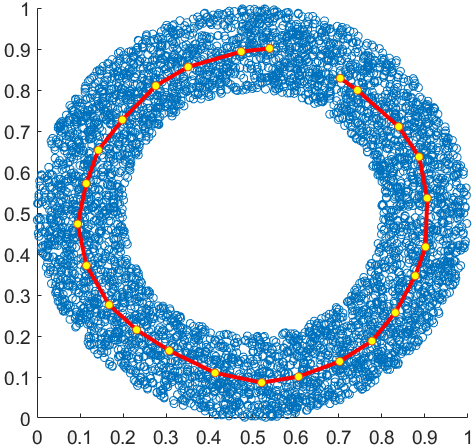
\includegraphics[width=0.8\linewidth]{figures/1d.png}
  \caption{1D SOM - 25 neurons, iterations = 15000, learning rate = 0.1, radius = 3.}
  \label{fig:1d}
\end{figure}

\begin{figure}[!h]
  \centering
  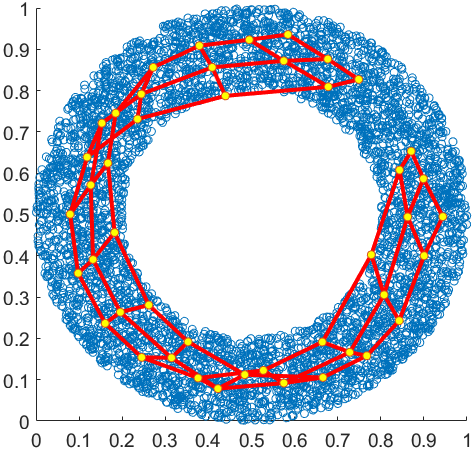
\includegraphics[width=0.8\linewidth]{figures/2d.png}
  \caption{2D SOM - 15x3 neurons. iterations = 15000, learning rate = 0.1, radius = 3.}
  \label{fig:2d}
\end{figure}

\section{Image clustering with SOM}

After training the SOM with default parameters, I produced Figure \ref{fig:u}. Unified distance matrices are used to represent high-dimensional data in a 2-dimensional image by visualizing the distances between neurons. This is useful because the distance between neurons is descriptive of the distance between data points, since the neurons' weight is influenced by the data points' locations. Similar colors show clustering as they are indicative of closely related neurons, while different colors represent larger distance between neurons. 

Based on the U-matrix, the SOM is trained to find images which have a cluster of similar colors in the middle, which is indicative of an image with a single object in the middle. This is based on the color clustering in the middle of the matrix. With the default parameters, it works in some cases, but often finds images which do not have an object in the middle. Increasing the training steps a hundred fold for both rough and finetune training significantly improves the results and produces the U-matrix in  Figure \ref{fig:u2}. Changing the map size resulted in no observable difference in accuracy. It added just as many similar images as it did random non-similar images. Unless, of course, the SOM has become better capable of detecting similarities than me - a human.

\begin{figure}[htbp]
\begin{minipage}[t]{0.45\linewidth}
  \centering
  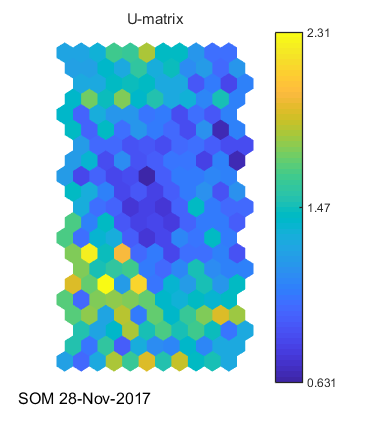
\includegraphics[width=\linewidth]{figures/U-matrix.png}
  \caption{U-matrix with default parameters.}
  \label{fig:u}
\end{minipage}%
    \hfill%
\begin{minipage}[t]{0.45\linewidth}
  \centering
  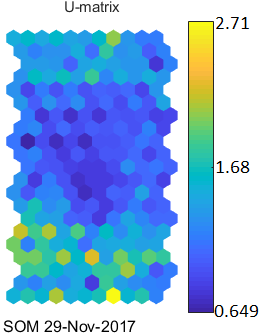
\includegraphics[width=\linewidth]{figures/U-matrix2.png}
  \caption{U-matrix with 100x default training steps.}
  \label{fig:u2}
\end{minipage} 
\end{figure}

\end{document}